% 论文正文是主体,主体部分应从另页右页开始,每一章应另起页。一般由序号标题、文字叙述、图、表格和公式等五个部分构成。
\section{绪论}
\subsection{研究背景与意义}

``人类基因组计划”的研究引发后基因组时代的到来,标志着生命科学开始进入系统生物学时代,人们开始研究各种组学在DNA、mRNA、蛋白质和各种代谢产物水平上研究各种分子的生物功能。
系统生物学首先通过生物学技术对系统进行干涉,并利用物理、化学实验方法测量得到实验数据,
然后将这些数据用计算机存储起来,最后运用数学、物理方法结合计算机技术对这些数据进行统计、分析,利用数学理论建立生物系统模型。
所以系统生物学研究的的方法和手段,决定了系统生物学是一个物理、化学、数学、信息学、计算机科学和分子生物学等多学科交叉学科,需要各种学科的密切配合\cite{ideker2001new}。

在系统生物学上,基础和核心问题是理解和认识能够代表基因发育和调控过程因果关系的基因调控网络~(GRNs, Gene Regulatory Networks)。
基因调控网络描述的是细胞或组织内复杂的生命过程中的功能通路,比如新陈代谢、基因调控、运输机制或者信号传导。
从宏观看,基因调控网络是由细胞中参与基因调控作用的~DNA、RNA、蛋白质~(protein)~以及代谢中间物所形成的相互作用的网络~\cite{de2002modeling}。
从微观看,一个基因的转录由细胞的生化状态所决定,在一个基因的转录过程中,一组转录因子作用于该基因的启动子区域,
控制该基因转录,而这些转录因子本身又是其它基因的产物。
当一个基因通过转录、翻译形成功能基因产物后,它将改变细胞的生化状态,
从而直接或间接地影响其它基因的表达或者自身的表达。
多个基因的表达不断变化,使得细胞的生化状态不断地变化,构成复杂的基因调控网络。

问题建模上,基因调控网络可以用来描述分子实体之间的相互依赖关系,可以用图结构中的有向无环图~(DAG,directed acyclic graph)~来表示,如图~\ref{cover-1}所示。
节点表示基因、蛋白质、代谢物质或者~RNA, 边代表的是分子实体间的关系,如蛋白质-DNA、蛋白质-蛋白质的相互作用关系或者其它关系,如图~\ref{cover-2}所示。
\begin{figure}[!htbp]
    \centering
    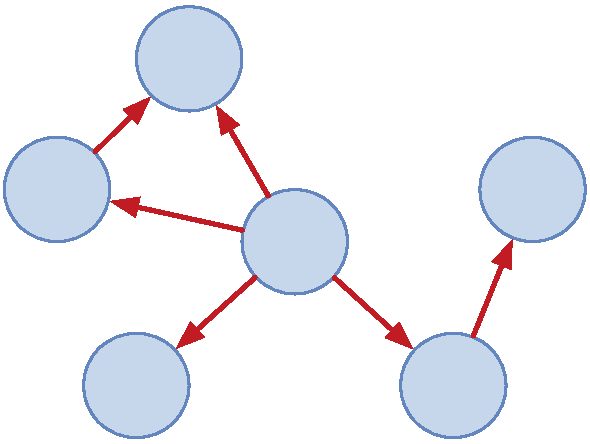
\includegraphics[width=0.75\textwidth]{cover-1.pdf}
    \caption{GRNs~拓扑结构示例图, 其中节点代表生物化合物, 节点边代表它们之间的关系。
    }
    \label{cover-1}
\end{figure}
\begin{figure}[!htbp]
    \centering
    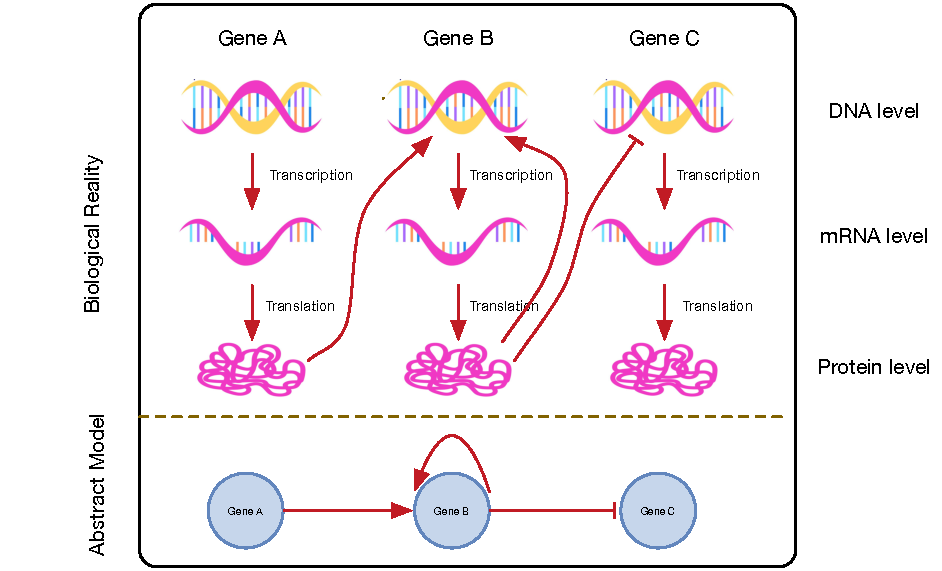
\includegraphics[width=0.95\textwidth]{cover-2.pdf}
    \caption{GRNs~构建的主要目标是为实际生物过程生成抽象模型。
    这些模型试图表示生物过程分子实体之间复杂的相互作用,比如基因激活、抑制或反馈环路。
    }
    \label{cover-2}
\end{figure}

微阵列芯片~(microarray)~技术和单细胞~RNA测序~(scRNA-seq)~技术的发展产生的大量基因表达数据,
这些基因表达数据不仅可用于分析基因表达的时空规律,研究基因的功能,而且还可用于基因之间的相互制约关系,研究基因调控网络模型,为理解生物潜在的调控机制带来了机遇。
另外, 转录组学、蛋白质组学、相互作用组学、代谢组学等高通量的实验室技术可以为模型提供更多的先验信息,有助于构建更加复杂、更准确地反映生命现象的基因调控动态网络。

% 基因调控网络建模(构建)是当前生物信息学研究的重要领域和关键问题。
% 构建基因调控网络,需要利用基因表达数据来学习和挖掘基因间的调控关系,并借助于可视化技术展现基因调控网络的拓扑结构,进一步可促进基因功能的新发现和疾病相关的潜在基因的预测 \cite{lee2009computational}。

基因调控网络的构建,立足于阐明基因表达调控的作用关系,
有利于从网络的角度去了解复杂而精密的生物网络系统所蕴涵的结构和功能信息,
彻底了解网络的生物学意义,节省大量的实验费用与资源,
也可以利用模拟结果有效地指导进一步的生物实验,更好地了解生物系统的功能,
尤其是在肿瘤等复杂疾病研究中,
例如癌症细胞的分化、扩散和增生等~\cite{hurley2011gene}。
通过基因调控网络建模,分析细胞代谢通路,在分子水平上理解癌症发生的机理,揭示癌症的内部机制,将进一步增强对癌症的整体认识,
发现诊断、控制和治疗癌症的方法~\cite{kreeger2009cancer,yan2016biological}。
此外,基因调控网络建模还有助于肿瘤药物的筛选和研制,能为攻克癌症等复杂疾病做出贡献。

总之, 基因调控网络建模是一门理论研究与实践应用相结合的学科,它不仅有重要的学术意义,还有很高的商业价值,以及广阔的发展前景。
随着后基因组时代的到来,基因调控网络不仅可以为生物信息学提供大量的研究线索,
也可为特定生物问题提供强有力的理论依据,还可在疾病诊断、药物筛选等领域发挥更加广泛的作用~\cite{kreeger2009cancer}。

\subsection{国内外研究现状和发展动态}

基因调控网络建模是一种依靠数据挖掘进行的逆向工程研究, 即根据基因表达数据推理基因调控网络中的各类拓扑结构。
它首先通过生物实验获取高通量生物数据, 然后根据生物网络的先验知识,针对特定生物问题建立数学模型, 并设计合理的算法构建基因调控网络,
最后通过生物学实验验证逐步逼近和发现真实的基因调控网络~\cite{sima2009inference}。
从计算角度讲,基因调控网络推断依赖于已知的知识数据库发现~(KDD, Knowledge Database Discovery)~工作流程。
KDD~从输入数据预处理到模型的验证,通过数据库搜索比较之前的实验数据结果来完成的,如图~\ref{cover-3}~所示。
\begin{figure}[!htbp]
    \centering
    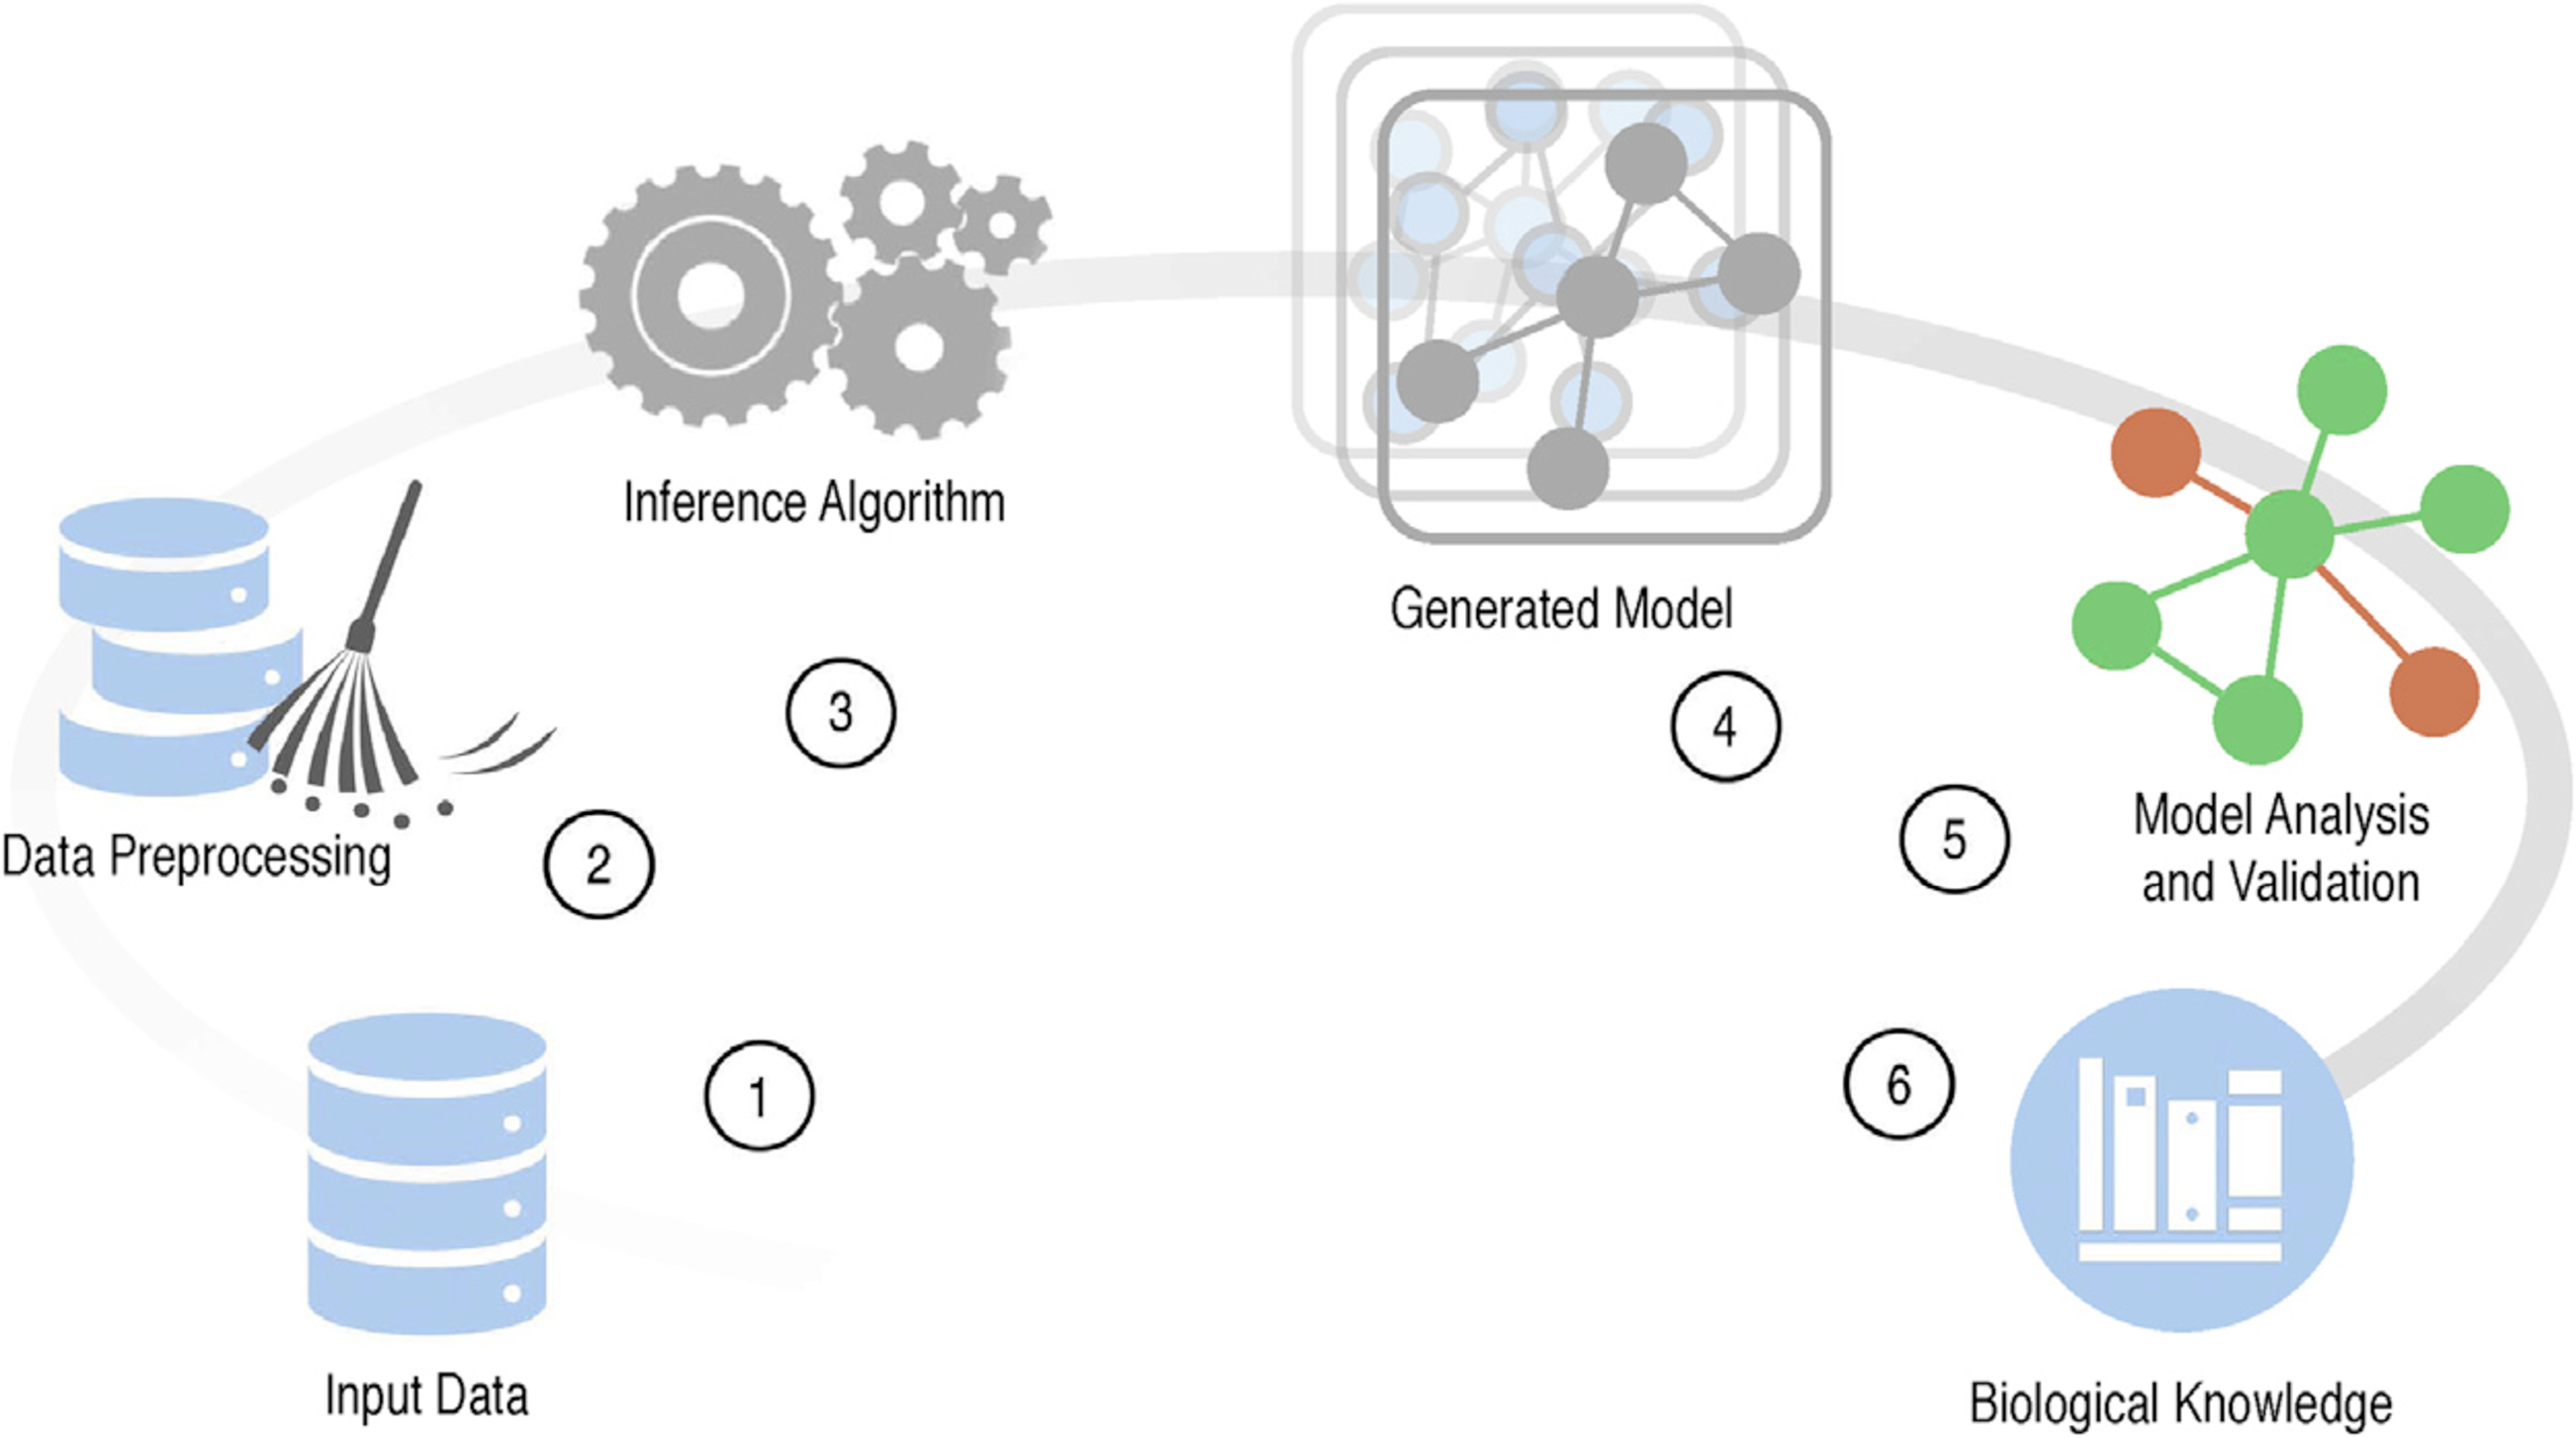
\includegraphics[width=0.95\textwidth]{cover-3.pdf}
    \caption{基于~KDD~工作流程的~GRN~重建步骤。
    \textcircled{\raisebox{-0.9pt}{1}}输入数据。
    \textcircled{\raisebox{-0.9pt}{2}}数据预处理。
    \textcircled{\raisebox{-0.9pt}{3}}网络推断算法。
    \textcircled{\raisebox{-0.9pt}{4}}生成模型。
    \textcircled{\raisebox{-0.9pt}{5}}模型分析和校验。
    \textcircled{\raisebox{-0.9pt}{6}}生物知识。
    }
    \label{cover-3}
\end{figure}

当前的基因调控网络建模牵涉到三方面的研究问题~\cite{schlitt2007current}:
\begin{enumerate}
    \item 建立什么样的模型;
    \item 如何设计与实现网络建模算法;
    \item 如何评价和甚至是应用构建的网络。
\end{enumerate}
下面将从前两个方面讨论基因调控网络建模的相关研究现状,
同时由于大多数方法是跟数据特性密切相关因此我们也需要介绍下数据源及其特征。

\subsubsection{数据源}
高通量技术提供了巨大的数据,诸如下一代测序技术~(NGS,Next Generation Sequencing)~\cite{BUERMANS20141932}, 
在过去十几年中产生了显著质量、稳健性和低噪声的~DNA~和~RNA~样本数据。
测序已经成为一种标准方法,被认为是研究生命体的基石~\cite{CEREB2015923}。
测序产生的基因表达数据使生物学家能够大规模观察基因的表达水平, 对推断基因调控网络起到了至关重要的作用。
基因表达数据来源包括~DNA~微阵列, RNA-seq~\cite{morin2008profiling}和~SAGE~(基因表达系列分析)~\cite{velculescu1995serial}。
用于基因调控网络构建的基因表达数据按照类型可以划分为时间序列数据~(time series data)~和扰动实验数据~(perturbation experiments data)~两种。
时间序列表达数据使生物学家能够调查生物网络中的时间模式;扰动表达数据提供了关于基因间调控方向的信息。
扰动实验分为两类:基因操作~(即基因缺失,过度表达,温度敏感或动力学突变)~\cite{holstege1998dissecting}~或外部处理~(即环境胁迫)~\cite{gasch2000genomic}。
在基因调控网络构建中我们将主要使用~DNA微阵列数据~(microarray data)~和单细胞~RNA-seq~数据~(scRNA-seq),同时也会结合其它比如~PPI~数据,~TF~结合位点数据等作为先验知识。

(1) DNA~微阵列测序数据

生物微阵列又被广泛地称为生物芯片,是上个世纪~90~年代以来最为重要的基因测序技术之一,
其技术的关键点是将巨大的~DNA~分析缩小到芯片上, 在利用光电技术对信号进行探测, 最后通过计算机加以分析。
借助基因芯片技术研究者可以测定基因在某一器官不同条件下不同发展阶段和不同组织中的转录水平,
从而建立基因表达谱以描绘基因组中的基因表达水平。
各种微阵列技术中, 用的最多的是基因微阵列芯片。
DNA~微阵列测序数据最为常见, 使用微阵列测序数据进行基因调控网络构建也历史悠久源远流长。

(2) 单细胞~RNA-seq~数据

单细胞~RNA-seq~技术在~2009年首先由~Tang等~\cite{tang2009mrna}提出,
但是在~2014~年以后由于新的协议和相对低廉的测序成本使得它在产业界和学术界都颇受欢迎,风靡至今。
单细胞~RNA-seq~技术与~DNA~微阵列测序技术最为显著的不同是,
后者测量的基因表达值是多个细胞基因表达值的平均值,
而前者测量的是单个细胞中的基因表达值。
单细胞~RNA-seq~测序技术也给数据处理带来诸多挑战,
比如大量的细胞异质性~\cite{wagner2016revealing},高度稀疏性导致的表达为零~(dropout)~\cite{kharchenko2014bayesian}, 细胞与细胞之间的测序深度变化, 细胞周期相关的批量效应~(batch effects)~\cite{buettner2015computational}。
在数据预处理阶段, 需要实现的目标不同和数据产生的场景, 对基因的~dropout值进行过滤或者填充~(dropout imputation), 或者需要对数据进行批量校正~(batch effects correction), 以提高后续下游分析的稳定性。
单细胞~RNA-seq~技术可以用来研究在转录组细胞特异性的变化中重要和新的生物学问题,
如鉴定细胞类型, 研究基因表达的随机性, 细胞发育轨迹推断,与细胞类型或者周期相关的基因调控网络的推断。
相比于批量测序数据而言, 大多数情况下单细胞~RNA-seq~数据的计算分析需要开发新的方法。

\subsubsection{网络模型}
寻找一个合适的网络模型是构建网络的首要问题。
在基因调控网络的研究中,为刻画和反映复杂生物网络的动态或静态行为,数学模型提供了一个强有力的工具。
不同的数学模型对基因调控网络进行了不同的表达和抽象,然而针对复杂的基因调控网络,
为对其进行全面描述,需要借助多个层次多种类型的模型来反映基因调控网络的不同特性。

从时空特性上区分,基因调控网络模型可分为:
静态模型与动态模型,例如,动态贝叶斯网是动态模型;
从建模所用的数据区分,模型可分为:
离散模型与连续模型,时序模型与非时序模型,例如对时序~(time-course)~数据可采用微分方程模型建模;
从图论角度区分,分为有向图模型和无向图模型;
从网络拓扑特性的角度出发,可构造出复杂网络和差异网络的模型。

模型改进和模型组合是当前网络模型的主要研究方向。
模型改进是针对现有的模型引入新的法则来构造新的模型,
而模型组合则是结合几个不同类型的模型取长补短达到性能最优。

\subsubsection{网络建模算法}
基因调控网络的各类模型都在不同层次、不同程度上对真实的调控网络进行了抽象,
下面针对关联网络、布尔网络、微分方程、贝叶斯网络、动态贝叶斯网络、回归方法的主要思想、优缺点以及研究进展做简要介绍。

(1) 布尔网络

布尔网络与微分方程相比则更为抽象,它对基因的状态做了进一步的简化,
用布尔函数代替了微分和导数来描述基因间的相互作用关系。
其中,基因的状态定量为两种不同的状态(``开"和``关")。
状态``开"表示一个基因转录表达, 状态``关"则代表一个基因未转录。
如果布尔网络模型进一步推广, 其可转变为时序布尔网络模型~TBN~(temporal Boolean networks), 这有利于处理多于一个单位时间跨度的基因间的依赖性。

基于布尔网络模型的主要工作包括: Kauffman~\cite{kauffman2003random}~提出布尔网络的分析框架;
Akusu~等~\cite{akutsu1999identification}~证明了布尔网络推理所需要的最少样本数量;
Liang~等~\cite{liang1998reveal}~开发了~REVEAL~算法。
Shmulevich~等~\cite{marshall2007inference}~将马尔可夫链~(Markov Chains)~和布尔网络结合起来,引进了概率布尔网络模型~PBN~(probabilistic boolean networks),
比标准布尔网络模型有了更多的优越性。
在单细胞~RNA-seq~测序数据上,
Chen~等~\cite{chen2014single}~开发了~SingleCellNet,
采用遗传算法从预期的轨迹通过细胞状态构造概率布尔模型, 他们采用的布尔规则直接来源于文献。
Moignard~等~\cite{moignard2015decoding}~提出了~SCNS~算法,通过状态转换图分析轨迹来推断一个异步布尔模型。
连接状态转换图在这个算法中起着至关重要的作用,但是它很难从单细胞表达数据中获取。

布尔网络建模时, 把基因的表达水平离散化成单一的表达和不表达两个数值,
而在现实的生物系统中,基因的表达过程是连续的,
对基因数据进行离散化时不可避免的会丢失很多重要的表达信息;
网络中一个节点更新,会使得所有节点同步更新,而在实际的基因表达过程中,更新是异步进行的。

(2) 微分方程模型

微分方程模型是一种连续的确定模型, 具有强大灵活的优点,
通过抽象基因间的时序调控变化,相比布尔网络来讲, 适合描述更加精细的调控关系,可以较好地建模基因表达数据。
另外,通过加入新的变量,微分方程模型可以进一步描述环境变化对于基因表达水平的影响。
微分方程的缺点则是难以适应中大型网络的构建, 中大型网络结构估计的精度较低,
样本数量要求严格,缺乏抗噪声能力、计算量较大, 捕捉基因表达数据中包含的随机信息欠佳。

若采用变量~$e_i$~表示第~$i$~个基因在~$t$~时刻的表达水平, 则~$n$~个基因之间的调控关系可以用微分方程描述如下:
\begin{equation}
\frac{{d_{e_i}}}{{dt}} = f_i (e),1 \le i \le n
\end{equation}

式中~$\frac{{d_{e_i }}}{{dt}}$~代表基因调控网络建模中,
第~$i$~个基因在~$t$~时刻表达水平的变化率,向量~$e=[e_1,e_2,...,e_n]^T$~则描述基因表达水平。
式中~$f_i(e)$~的表现形式表明了基因之间的调控机制和作用方式,也就是调控网络的结构。
调控函数~$f_i(e)$~最简单的形式是线性函数,可以表示为:
\begin{equation}
\frac{{d_{e_i }}}{{dt}} = \sum\nolimits_j {w_{ij} e_j} { + b_i } ,1 \le i \le n
\end{equation}

调控网络系统中各个基因之间的调控关系可采用参数~$w_{ij}$~表示,
激活、抑制和无调控关系分别对其取值为正、负或为零, $b_i$~表示基因的基础活性。
基因之间复杂的非线性作用关系可利用非线性的调控函数~$f_i(e)$~进行刻画和说明。
比如~Sigmoid~函数~(S型函数),来引入必要的非线性,具体表达形式为:

\begin{equation}
\frac{{d_{e_i } }}{{dt}} = AS(\sum\nolimits_j {w_{ij} e_j } + b_i) - D_i e_i ,1 \le i \le n
\end{equation}

Chen~\cite{chen1999modeling}~最早使用微分方程系统作为基因表达调控网络模型,
微分方程其主要的优点在于强大灵活,有利于描述基因网络中的复杂关系,能够很好的表现出基因之间的连续动态关系。
而其缺点在于生物学实验过程中蛋白质的含量比较难以获得,另外也忽略了其他调控物的影响,不能处理实验数据噪音问题。

在单细胞测序数据集上, 
为了从时间序列数据构建网络,SCODE~\cite{matsumoto2017scode}~和~SCOUP~\cite{matsumoto2016scoup}~
分别引入~ODEs~和~SDEs~来计算基因之间的相关性。
SCODE~将基因之间的相关性表示为控制基因表达水平随时间的分化的变量。
通过将某一基因在某一时间点的基因表达水平建模为对其他基因表达水平的线性依赖关系,
SCODE~使用线性回归来估计相关矩阵。
SCOUP~则将各基因表达水平随时间的分化建模为一个连续的随机扩散过程, 即~Ornstein-Uhlenbeck~(OU)~过程。
在该模型中,某一基因在某一时间点的表达量可以通过当前~OU~过程的正态分布来估计。
利用计算出的所有细胞的~z~值得到基因之间的相关性。

(3) 贝叶斯网络

贝叶斯网络~(Bayesian Networks, BNs)~是一种重要的概率模型,
由条件概率分布和网络结构两部分组成。
自从~Friedman~等~\cite{friedman2000using}~将贝叶斯网络应用到基因调控网络的重构中后,
贝叶斯网络在生物学上的应用越来越广泛,成为现今构建细胞调控网络最有效的方法之一。
在贝叶斯网络模型中变量之间的结构用有向无环图~(directed acyclic graph,DAG)~来表示,
变量之间的关系使用联合概率分布来描述。
相对于布尔网络的粗放定性,微分方程的精细定量,贝叶斯网络模型可看作这两者的折衷。

~Cooper等提出的~K2~算法~\cite{cooper1992bayesian}~是一个基于搜索评分的经典算法,
该算法为评价模型与数据的符合程度,
首先在给定先验信息和节点顺序的情况下,通过后验概率作为评分标准并利用贪婪搜索方法找出最佳网络结构。
%Peer~\cite{pe2001inferring}等人将贝叶斯网络技术用来处理调控网络中的扰动。
% 他们首先将数据离散化后根据评分函数挑选出最佳的的基因网络。
Imoto~等~\cite{kim2003inferring}~用非参数回归模型来解决离散化造成的阀值选取与信息丢失问题,
Imoto~等采用这一模型能获得基因之间的线性与非线性结构特征。
Jansen~等~\cite{jansen2003bayesian}~为利用贝叶斯网模型构建调控网络,
分析和计算各类基因表达数据以及蛋白质相互作用数据,并通过生物实验验证了模型的预测结果。
2004年~Friedman~等~\cite{friedman2004inferring}~为构建静态基因调控网络,
首次基于微阵列数据将贝叶斯网络模型用来预测基因调控关系。
Hartemink~等~\cite{hartemink2005reverse}~采用~BDe评分测度作为学习的目标函数,
通过对基因表达数据进行离散化及模拟退火算法来构建基因调控网络。
Werhli~和~Husmeier~\cite{werhli2007reconstructing}~将基因表达数据与来自多种数据源的先验生物学知识结合起来使用贝叶斯网络模型利用马尔科夫链蒙特卡洛~(MCMC)~抽样方案来抽样来自后验分布的超参数,
这种与多数据源的结合降低了基因调控网络参数学习的误差率,提高基因调控网络重建的准确性。
Yavari~等人~\cite{yavari2008gene}~根据基因本体将基因进行聚类,
并使用贝叶斯网络推断共聚簇基因之间的相互作用。
这种方法可以解决由于基因数目增加而导致的结构数量指数增加的问题。 
此外,他们还提出了一种在推理过程中使用共聚基因之间的互相关性的新方法。
共聚簇基因之间的互相关性为贝叶斯网络提供了时间延迟信息。 
由此模型产生的精度和灵敏度均有提高,而且结果表明这种模型适合对大规模基因进行建模。
杨等人~\cite{yang2011bayesian}~建议使用稀疏图搜索~(SGS)~算法减少贝叶斯网络的计算时间。
SGS算法利用迭代统计独立性测试和搜索技术来寻找最佳的网络结构。
最佳的基因调控网络是使用搜索-打分和基于约束两种方法混合产生的。
基于搜索和打分是使用优化技术在所有候选网络上搜索最佳网络结构并打分用来评估网络质。
基于约束的方法通过应用条件独立性检测来取代传统的统计或信息论度量来检测边的存在。
结果表明,他们提出的方法提高了准确性和计算效率。
Tan~和~Mohamad~\cite{kunga2012using}~使用贝叶斯网络结合爬山法和~Efron~的~bootstrap~抽样方法来构建基因调控网络。
他们首先使用最小局部平方~(LLS)~插值算法来处理微阵列数据集中存在的缺失值, 
然后采用贝叶斯网络建立网络模型并采用爬山算法进行学习, 
bootstrap~抽样方法被用来抽取高置信度的边集合。
他们的基因调控网络构建方法获得了较高的真阳性率, 并且揭示了基因之间更新的关系。 
Young~等~\cite{young2014fast}~提出一种基于贝叶斯网络的~ScanBMA~算法,
该方法采取数据变换和新的策略在模型空间搜索时高效快速,
可应用于大规模的基因调控网络推断。

贝叶斯网络模型的优点是灵活性好, 具有从数据中推导模型的能力, 能够自然地融入先验知识并能用专家知识和数据挖掘来改进模型的性能;
可以通过借助问题领域自身结构特征和变量间直接影响的局部性, 同时使用条件独立的数学概念, 将聚合概率分布的计算问题,分解为若干局部条件概率分布的计算问题;
模型结构和参数具有明确的含义可解释性好, 具有良好的学习能力; 能很好地处理隐变量和数据缺失问题。
研究发现与关联网络相比, 贝叶斯网络在识别准确度上常有更优异的表现, 尤其是在网络规模较小时。
其不足之处是:许多贝叶斯网和动态贝叶斯网常采用离散模型, 对基因表达数据离散化导致损失了部分信息,
同时也降低了网络建模的准确度;
没有时序的概念,特别是对于存在伪时序的单细胞数据集而言,不能明显地表现基因调控网络的动力学特征。

(4) 动态贝叶斯网络

动态贝叶斯网络~(Dynamic Bayesian Network,DBN)~模型是在静态~BN~网络模型中引入时间因素而形成的动态网络~\cite{dondelinger2010heterogeneous,grzegorczyk2010improvements}。
DBN~可以很好的表示随机系统的动态特性,也使用图模型的方式来表示模型中随机变量之间的概率依赖关系~\cite{hecker2009gene}。
DBN~更好地刻画了基因调控网络的动态特性,善于处理非线性关系和由随机现象引起的不确定性,能够描述基因之间的负反馈调控过程,
相比于静态贝叶斯网它能够克服其有向无环的缺点,具有很好的概率推理能力和知识表达能力,使得模型的预测精度进一步提高。

Friedman~和~Murphy~等~\cite{friedman2004inferring}~考虑到了基因调控存在一定的时延性,
从理论的角度分析了~DBN~从时序基因表达数据构建基因调控网络的问题, 提出用动态贝叶斯网络模型分析时序基因表达数据。
Smith~等~\cite{smith2006computational}~用动态贝叶斯网络模型来分析微阵列数据,
结合了基因调控的负反馈与时延因素, 因此需要采用网络中不同节点来表示同一基因不同时间点的表达向量。
Wu和Liu等~\cite{wu2008dynamic}~改进了动态贝叶斯网络建模方法,使用了~MCMC~和带重启的贪心爬山算法两种不同的模型搜索方法。 
两种方法在时间效率上不相上下,与带重启的贪心爬山算法相比~MCMC~具有更高的预测精度。
Song~\cite{song2009keller}结合微阵列数据与基因关系的先验知识在~DBN~上提出新的数据整合模型,利用并行算法,构建基因调控网络。
Kim~等~\cite{del2010efficient}~也在这方面做了大量的工作,
并结合线性或非线性模型以及相应的生物学知识对动态贝叶斯网络进行了改进。
Norbert~\cite{netrapalli2010greedy}~为从基因扰动型实验数据中学习动态贝叶斯网络,
利用~Husmeier~\cite{werhli2006comparative}~提出的离散化方法来对基因表达数据进行预处理,
并使用~BDe~测度来进行评分搜索,最终构建动态贝叶斯网络, 这种搜索方法实现了减少学习时间,降低计算的时间复杂度的目的~\cite{hurley2011gene}。
Grzegorczyk~和~Husmeier~\cite{grzegorczyk2010improvements}~通过将多变点过程与可逆跳跃马尔可夫链蒙特卡罗方法~(RJMCMC)~结合,改进了基于动态贝叶斯网络推断的方法。 他们通过引入动态编程方案来优化RJMCMC上的收敛性,该方法从正确的条件分布对变化点进行采样。 
此外,引入了贝叶斯聚类的新方法以促进节点之间的信息共享, 使得模型复杂度能够自动调整。
Chai~等~\cite{chai2012inferring}~提出了缺失值插补的动态贝叶斯网络模型,
利用缺失值插补来提高基因调控网络推断中的计算效率,
同时通过限制潜在调控因子的表达变化来缩短计算时间。
Vinh~等~\cite{vinh2012gene}~将动态贝叶斯网络方法与基于时间序列表达数据的基因调控网络构建的全局最优化相结合,
他们在全局优化框架上使用互信息测试来学习高阶带延时的基因相互作用。
他们的方法能够改善动态贝叶斯网络只适合于小规模网络的缺陷,
同时能够避免动态贝叶斯网络结构学习容易陷入局部最优的状况。

(5) 关联网络

关联网络~(relevance network)~主要借助基因表达数据间相关性的计算来构建模型。
相关性分析是构建基因调控网络最常见的方法之一。
计算基因间的相关性常通过互信息、皮尔逊相关系数等测度来进行。
主要思路是: 对于预先设定的阈值, 若基因间相关性不在阈值范围内, 则在网络中基因间有边相连。
若两基因间具有相同或相近的调控机制, 则两个基因相关性较高,
尤其是,对于同一转录因子的靶基因或同一条生物通路上的基因,它们的相似度或相关性较高。

皮尔逊相关系数~(PCC)~是一种线性相关系数, 它反映了两个变量间的线性相关程度。
设~$X$, $Y$~为随机变量, $pcc(X,Y)$~定义如下:

\begin{equation}
pcc(X,Y) = \frac{{\sum\limits_i {(x_i -\bar x_i )(y_i -\bar y_i )} }}{{\sqrt {\sum\limits_i {(x_i  - \bar x_i )^2 } } \sqrt {\sum\limits_i {(y_i  - \bar y_i )^2 } } }}
\end{equation}

其中,$\bar x_i$、$\bar y_i$~分别是~X、Y~的均值。
$pcc(X,Y)$~的取值在~-1到~1之间。
当~$pcc(X,Y)$~为~-1~或者~1~时, 表示两个变量完全相关;
当~$pcc(X,Y)$~为~0~时, 表示两个变量完全无关。

PCC~被广泛用于评估变量之间的线性关系~\cite{stuart2003gene},但在不借助其他信息的情况下无法区分直接关系和间接关系,而偏相关分析法~(PC)~\cite{baba2004partial}~通过考虑附加信息条件来有效区分直接和间接关系。
另外, Barabási~等~\cite{barzel2013network}~提出了一个基于动态关联性的方法,该方法通过消除网络中的间接影响进行直接关联性和间接关联性区分; 
Feizi等~\cite{feizi2013network}~提出了利用网络卷积去除所有关联之间的综合效应区分直接和间接关联性。
这两种方法~\cite{barzel2013network,feizi2013network}~只能测量线性直接关联性,
但无法测量非线性关联性, 而非线性关联性在许多非线性系统比如生物系统中发挥着重要的作用。
基于~PCC~和~PC, 距离相关性~\cite{szekely2007measuring,kosorok2009brownian}~和部分距离相关性~(Pdcor)~\cite{szekely2014partial}~被提出用于度量随机向量间的相关性,这些统计量对于依赖偏离很敏感。
Pdcor~的评估存在假阳性,即当向量~$X$~非条件独立时, Pdcor(X;Y|Z)~也有可能为零~\cite{szekely2014partial}。


互信息~(Mutual Information)~常用来刻画和描述两个系统间的统计相关性,或通
过熵来反映一个系统中蕴含的另一个系统信息量的大小, 设~$P(x)$~是~$X=x$~的概率,
则随机变量~$X$~的熵定义为~\cite{cover2012elements}:
\begin{equation}
H(X) = - \sum\limits_x {P(x)\log _2 P(x)} 
\end{equation}

设$P(x,y)$是$X=x$,$Y=y$ 时的联合概率,则$X$,$Y$的联合熵定义为:
\begin{equation}
H(X,Y) =  - \sum\limits_x {\sum\limits_y {P(x,y)\log _2 P(x,y)} } 
\end{equation}

随机变量~$X$~和~$Y$~的互信息为:
\begin{equation}
MI(X,Y) = H(X) + H(Y) - H(X,Y) = \sum\limits_{i,j} {P(x_i ,y_i )\log \frac{{p(x_i,y_i )}}{{p(x_i )p(y_i )}}} 
\end{equation}

需要注意的是在基因调控网络推断中由于基因表达数据是连续的,而互信息在计算时需要离散化,
一般使用~B-样条平滑和离散化方法来进行计算~\cite{daub2004estimating}。
由于互信息能够捕获有效捕获变量间的非线性相关性,
因此在复杂的基因调控网络相互作用推断中其应用十分广泛~\cite{brunel2010miss,zhang2011inferring}。

Butte~等~\cite{basso2005reverse}~首先利用互信息计算所有基因对之间的相关性,然后设置互信息阈值。
为构建关联基因调控网络, 通常定义高于阈值的基因对之间存在关联并使用边连接起来构成网络。
Margolin~等~\cite{margolin2006aracne}~提出的~ARCANE~采用~Data Processing Inequality~(DPI)~来过滤间接作用边。
Faith~等~\cite{faith2007large}~提出的~CLR~方法使用互信息的经验分布来过滤间接作用边。
Meyer~等~\cite{meyer2007information}~提出的~MRNET~方法使用最小化冗余特征选择算法~\cite{peng2005feature},
在计算后的互信息网络上对每一个目标基因选择一个同目标基因关联最强但与已经候选的基因集合冗余性最低的基因,这个过程不断进行迭代。
Altay~等~\cite{altay2010inferring}~提出的~C3NET~和其扩展算法~BC3NET~\cite{de2012bagging}~结合一个最大化的步骤来估计互信息从而使预测更准确。

MI~被广泛用于评估变量之间的非线性相关性,
该方法基于统计独立性在只有联合概率信息时无法计算直接关联性或依赖性,
并且和~PCC~一样有假阳性~\cite{frenzel2007partial,schreiber2000measuring}。
类似于~PC~和~PCC,~Zhao~等提出了条件互信息~(Conditional Mutual Information,CMI)~\cite{zhang2011inferring}~和部分互信息~(Part Mutual Information,PMI)~\cite{zhao2016part},
这两个测度在互信息上引入了条件计算的机制减少了假阳性边,
能有效检测变量之间非线性的间接或直接的相互作用。
他们将这两个参数与基于贪心策略的路径一致性算法~(Path Consistency Algorithm, PCA)~结合起来先后提出了~PCA-CMI\cite{zhang2011inferring}~和~PCA-PMI\cite{zhao2016part}。

在单细胞测序数据集上,
Yu~等提出了~NLNET~方法\cite{yu2013hierarchical}, 
两个基因之间的相关性被定义为基于条件有序列表~(Conditional ordered list,DCOL)~的距离,
其中基因~G1~到基因~G2~的距离取决于通过~G1~中所有样本的表达顺序。
NLNET使用的这种距离度量并没有考虑到真实生物网络中的一个基因可能与多个基因相互作用的事实。
Thalia~等~\cite{chan2017gene}~提出了高效的~PIDC~算法,
利用偏信息分解~(partial information decomposition,PID)~测度来衡量基因之间的关系。
Guo~等~\cite{guo2015sincera}~提出了~SINCERA~方法, 该方法利用低阶偏相关性~(low-order partial correlation),可以在测量中涉及两个以上的基因,是一种更符合实际的方式来呈现复杂网络的相互作用。
在~SINCERA~方法中,给定第三个基因~G3,基因~G1~和基因~G2~之间的相关性是~G1~与~G3~的线性回归
所产生的残差与~G2~与~G3~的线性回归所产生的残差之间的相关性。
SINCERA~使用最小平方估计来计算目标基因和条件基因的回归系数, 假设基因之间存在线性依赖关系。

可以看出,虽然关联网络建模操作简单易行,但不管是基于~PCC、MI~还是~PID~等构建的网络极其容易引进假阳性边。
虽然各种方法都站在不同的角度来尽量减少假阳性边来提高网络构建的准确性。
但是随着网络规模的扩大这种状况还是在不断恶化,网络构建的准确性急剧下降。

(6) 回归方法

近年来由于~DREAM~系列竞赛的推动,利用机器学习回归模型进行基因调控网络的构建方法大量涌现。
这类方法本质上可以看作是关联网络模型的延伸,
与关联网络只关注量化相互作用不同的是回归方法能够推断出基因之间的相互作用方向。
回归模型将基因调控建模转化为机器学习特征选择的问题,
即是将靶标基因的表达看作是调控基因表达之间的相互线性作用或者非线性作用的结果,
采用~bagging~或者~boosting~的做法,推断出最终的基因调控网络。
它们应用在基因调控网络构建上优点是计算效率高,网络构建准确率高,
缺点是一些非线性的模型可解释性较低参数意义不明确,缺少对生物结构的支持。
回归模型成功应用于基因调控网络构建中的典型算法包括基于随机森林的~GENIE3~\cite{Huynh-Thu2010},
基于~Lasso~回归的~TIGRESS~\cite{Haury2012}。
在处理时间序列数据上有~GENIE3的扩展方法~GENIE3-lag~\cite{huynh2012machine},
与扩散模型相结合利用随机森林来学习隐含参数的~Jump3~\cite{Huynh-Thu2014}。

在单细胞~RNA-seq~测序数据集上, 
SCENIC~\cite{aibar2017scenic}~融合了~GENIE3,RcisTarget~和~AUCell~三个算法来在单细胞测序数据上实现了基因调控网络的构建和基因的聚类。
单细胞~RNA-seq~也能产生基于时间序列的~RNA-seq~数据。
与传统的时间序列数据相比,基于单细胞的时序数据在单个时间片上将产生更多的样本, 但是这样测序代价会十分高昂。
因此也有很多方法利用原始数据推断出伪时序~(pseudo-time ordering)~后再利用回归方法构建基因调控网络。
LEAP~\cite{specht2017leap}~简单地使用皮尔逊相关性来计算每个时间窗口的基因之间的相关性。 
然后,它通过收集所有时间窗口内所有基因对的最大相关性来合并所有相关矩阵。
SINCERITIES~\cite{papili2017sincerities}~利用基因在不同时间片上的表达分布之间的距离来构建基因的表达矢量,
然后使用格兰杰因果关系~(Granger causality)~的思想结合线性回归模型来推断基因调控网络。
SINCERITIES~并没有直接来计算在每个时间窗口中的基因间的相关性。
SCIMITAR~\cite{cordero2017tracing}~使用连续的多变量高斯混合模型对数据进行建模,
然后使用期望值最大化~(EM)~算法估计参数。
EM~算法估计了每个分布的参数,以及一个细胞属于每个分布的可能性。
SCIMITAR~从混合模型的协方差矩阵中计算出每个伪时间的相关矩阵。
然后,该方法通过计算协方差矩阵之间的距离来计算相似度矩阵。
然后使用相似度矩阵的频谱聚类来确定整个时间轨迹的发展阶段。
对于每个发展阶段,该方法通过对该阶段的相关矩阵进行平均,输出共识网络。
SINGE~\cite{deshpande2019network}~使用回归模型来确定一个时间窗口内两个基因之间的相关性。
对于每个目标基因,该方法利用基于核函数的格兰杰因果关系~(Granger causality)~回归来计算该基因与所有其它基因的相关性(即边或连接)。
聚合时该方法采用~Borda~计数聚合法~\cite{van2000variants},
该方法偏重于多次格兰杰检验一致性排名靠前的连接,对两个基因之间的连接进行随时间的排序。
上述四种方法中, SCIMITAR~自身能直接从输入的数据中推断出细胞的伪时序, 
而~LEAP、SINCERITIES~和~SINGE~都依赖用户在输入时候提供细胞的时间排序。

\subsection{主要研究工作}
本课题的主要研究内容是基因调控网络构建的研究。
从系统生物学的角度出发,通过计算方法研究基于~DNA~微阵列数据以及
单细胞~RNA-seq~测序数据上的基因调控网络的构建、评估及其在复杂细胞类型分析等生物问题中的应用。
本项目以复杂网络理论、信息论和机器学习方法为基础,以数据的结构特性为研究对象,
提出合适的网络推断模型,提出基于不同表达数据的基因调控网络构建方法,
并同已有的方法进行对比评估。

(1) 基于互信息网络推断算法研究

通过对基于信息理论互信息的网络推断算法进行研究后发现,
由于原始数据中存在的外部噪声、
网络结构中的拓扑稀疏性和非线性基因之间的依赖等因素,
现如今基于此的这些方法在网络推断中会引入冗余的依赖关系。
特别是随着网络规模的增加,这些方法的表现大幅降低。
我们提出了一种新的网络结构推断方法~Loc-PCA-CMI:
首先识别局部重叠基因簇,
然后基于条件互信息~(PCA-CMI)~的路径一致性算法推断每个簇的局部网络结构,
最终通过聚合局部网络结构,也就是基因之间的依赖性网络,来构造最终的~GRN。

(2) 基于回归方法的数据驱动的网络推断算法研究

最近关于数据驱动的动态网络构建的研究为我们提供了解决回归问题的新视角。
在这项研究中, 我们提出了一种数据驱动的动态网络构建方法来推断基因调控网络~(D3GRN)。
其中,将每个目标基因的调控关系转化为功能分解问题,并利用揭示网络相互作用的算法~(ARNI)~解决各个子问题。
为了弥补~ARNI~仅从单元级构建网络的局限性,
我们采用抽样和基于面积的评分方法来推断最终的网络。


(3) 基于单细胞~RNA-seq~测序数据的稀有细胞识别和聚类算法研究

单细胞数据填充、聚类以及稀有细胞识别是单细胞数据上游分析的核心任务, 
在很大程度上与本研究的重点,也就是构建与细胞类型相关的基因调控网络的必要步骤。
现有的寻找稀有细胞的算法非常耗时或耗费内存。
本文中,我们提出了一种高效准确的方法~DoRC~(\underline{D}iscovery \underline{o}f \underline{R}are \underline{C}ells)。
DoRC~产生的稀有度分数可以帮助生物学家们着重于下游分析,只对超大规模内的部分表达单细胞~RNA-seq~数据进行分析。
为了在随后的下游分析的过程中区分细胞类型,我们提出了新颖有效的细胞聚类方法~RafClust。

(4) 基于矩阵分解的单细胞基因表达调控网络方法研究

识别细胞类型特征和细胞的基因表达活动程序~(如生命周期过程、对环境因素的反应)~对于理解细胞和组织的组成至关重要。
虽然单细胞~RNA-Seq~数据可以量化成单个细胞中的转录本,
每个细胞的表达谱可能是这两种类型的程序的混合物, 使它们难以分离。
在这里, 我们提出了一个使用矩阵分解的算法~WSSMFA~来解决这个问题。
通过模拟表明, 我们提出的~scGRNHunter~方法可以准确地推断出身份和活动性的子程序~(包括它们在每个细胞的相对贡献), 
并在此基础上构建基因调控网络。

\subsection{论文组织结构}

全文内容共六章,各章内容简述如下:

第一章~绪论。主要描述了基因调控网络研究在目前的研究背景与意义, 国内外研究现状和发展动态。
最后, 介绍本论文的研究内容, 并给出全文的结构安排。

第二章~基于互信息网络推断算法研究。主要介绍了基于互信息网络推断算法相关工作, 为了降低假阳性调控边的引入设计了
Loc-PCA-CMI~算法, 介绍了算法细节, 并对使用的数据集、使用的数据集、评价指标进行了介绍, 之后对实验结果进行了讨论和总结。

第三章~基于回归方法的数据驱动的网络推断算法研究。主要回顾了当前最热的基于回归的基因调控网络构建方法的研究现状,
对比了~D3GRN~与其它几种方法的设计思路, 并给出了~D3GRN~的算法细节, 并对使用的数据集、使用的数据集、评价指标进行了介绍, 之后对实验结果进行了讨论和总结。

第四章~基于单细胞~RNA-seq~数据的稀有细胞识别和聚类算法研究。主要回顾了当前稀有细胞识别方向的方法及其优缺点, 
DoRC~的设计思路以及~DoRC~方法详细的流程,针对过滤之后的稀有细胞后使用的~RafClust~聚类算法的实现细节, 基因差异分析。
之后详细介绍了实验结果, 并对实验结果进行了讨论和总结。

第五章~基于矩阵分解的单细胞基因表达调控网络方法研究。主要提出了一种新的单细胞数据上进行身份~GEP~(gene expressin program)~和活动~
GEP~进行构建的想法, 并以此为基础详细介绍了~scGRNHunter~的几个步骤, 其中重点介绍了矩阵分解算法~WSSMFA。
最后我们介绍了实验数据, 实验结果, 并对后续的研究进行了探讨。

第六章~总结与展望。总结全文并对未来的研究方向进行了展望。

% \newpage

% \section{图像与表格布局}
% \label{sec.figure}
% \textbf{按学校格式要求,每个子图的小标(a)、(b)、(c)等在【左上角】。}

% \subsection{单图布局}

% \lipsum

% \textbf{单图布局如图\ref{F.csu_single}所示。}

% \begin{figure}[hbt]
% \centering
% 
\includegraphics[width=0.5\textwidth]{csu.png}
% \caption{单图布局示例}
% \label{F.csu_single}
% \end{figure}

% \subsection{横排布局}

% \textbf{横排布局如图\ref{F.csu_row}所示。}

% \begin{figure}[!htb]
%     \centering
%     \begin{subfigure}[t]{0.24\linewidth}
%         \caption{}
%         \begin{minipage}[b]{1\linewidth}
%         
\includegraphics[width=1\linewidth]{csu.png}
%         \end{minipage}
%     \end{subfigure}
%     \begin{subfigure}[t]{0.24\linewidth}
%         \caption{}
%         \begin{minipage}[b]{1\linewidth}
%         
\includegraphics[width=1\linewidth]{csu.png}
%         \end{minipage}
%     \end{subfigure}
%     \begin{subfigure}[t]{0.24\linewidth}
%         \caption{}
%         \begin{minipage}[b]{1\linewidth}
%         
\includegraphics[width=1\linewidth]{csu.png}
%         \end{minipage}
%     \end{subfigure}
%     \begin{subfigure}[t]{0.24\linewidth}
%         \caption{}
%         \begin{minipage}[b]{1\linewidth}
%         
\includegraphics[width=1\linewidth]{csu.png}
%         \end{minipage}
%     \end{subfigure}
%     \caption{横排布局示例}
%     \label{F.csu_row}
% \end{figure}

% \lipsum

% \subsection{竖排布局}
% \textbf{竖排布局如图\ref{F.csu_col}所示。}

% \begin{figure}[!htb]
%     \centering
%     \begin{subfigure}[t]{0.15\linewidth}
%         \caption{}
%         \begin{minipage}[b]{1\linewidth}
%         
\includegraphics[width=1\linewidth]{csu.png}
%         \end{minipage}
%     \end{subfigure}\\
%     \begin{subfigure}[t]{0.15\linewidth}
%         \caption{}
%         \begin{minipage}[b]{1\linewidth}
%         
\includegraphics[width=1\linewidth]{csu.png}
%         \end{minipage}
%     \end{subfigure}
%     \caption{竖排布局示例}
%     \label{F.csu_col}
% \end{figure}

% \lipsum

% \subsection{竖排多图横排布局}

% \begin{figure}[!htb]
%     \centering
%     \begin{subfigure}[t]{0.13\linewidth}
%         \caption{}
%         \begin{minipage}[b]{1\linewidth}
%         
\includegraphics[width=1\linewidth]{csu.png} \vspace{-1ex} \vfill 
%         
\includegraphics[width=1\linewidth]{csu.png}
%         \end{minipage}
%     \end{subfigure}
%     \begin{subfigure}[t]{0.13\linewidth}
%         \caption{}
%         \begin{minipage}[b]{1\linewidth}
%         
\includegraphics[width=1\linewidth]{csu.png} \vspace{-1ex} \vfill 
%         
\includegraphics[width=1\linewidth]{csu.png}
%         \end{minipage}
%     \end{subfigure}
%     \caption{竖排多图横排布局}
%     \label{F.csu_col_row}
% \end{figure}

% \textbf{竖排多图横排布局如图\ref{F.csu_col_row}所示。注意看(a)、(b)编号与图关系。}


% \subsection{横排多图竖排布局}

% \lipsum

% \begin{figure}[!htb]
%     \centering
%     \begin{subfigure}[t]{0.3\linewidth}
%         \caption{}
%         \begin{minipage}[b]{1\linewidth}
%         
\includegraphics[width=0.45\linewidth]{csu.png}
%         
\includegraphics[width=0.45\linewidth]{csu.png}
%         \end{minipage}
%     \end{subfigure}\\
%     \begin{subfigure}[t]{0.3\linewidth}
%         \caption{}
%         \begin{minipage}[b]{1\linewidth}
%         
\includegraphics[width=0.45\linewidth]{csu.png}
%         
\includegraphics[width=0.45\linewidth]{csu.png}
%         \end{minipage}
%     \end{subfigure}
%     \caption{横排多图竖排布局}
%     \label{F.csu_row_col}
% \end{figure}

% \textbf{横排多图竖排布局如图\ref{F.csu_row_col}所示。注意看(a)、(b)编号与图关系。}


% \subsection{本章小结}
% 本章示例图片布局。

% \subsection{表格插入示例}

% \begin{table}[htb]
%   \centering
%   \caption{学校文件里对表格的要求不是很高,不过按照学术论文的一般规范,表格为三线表。}
%   \label{T.example}
%   \begin{tabular}{llllll}
%   \hline
%    & A  & B  & C  & D  & E \\
%   \hline
% 1 	& 212 & 414 & 4 		& 23 & fgw	\\
% 2 	& 212 & 414 & v 		& 23 & fgw	\\
% 3 	& 212 & 414 & vfwe		& 23 & 嗯	\\
% 4 	& 212 & 414 & 4fwe		& 23 & 嗯	\\
% 5 	& af2 & 4vx & 4 		& 23 & fgw	\\
% 6 	& af2 & 4vx & 4 		& 23 & fgw	\\
% 7 	& 212 & 414 & 4 		& 23 & fgw	\\

% \hline{}
% \end{tabular}
% \end{table}

% \textbf{表格如表\ref{T.example}所示,latex表格技巧很多,这里不再详细介绍。}

% \lipsum

% \newpage

% \subsection{公式插入示例}

% \lipsum

% \textbf{公式插入示例如公式(\ref{E.example})所示。}

% \begin{equation}
% \gamma_{x}=
% \left\{
%   \begin{array}{lr}
%   0, & {\rm if}~~\;|x| \leq \delta \\
%   x, & {\rm otherwise}
%   \end{array}
% \right.
% \label{E.example}
% \end{equation}

% \newpage